\documentclass[slideopt,A4,showboxes,svgnames]{beamer}

%% list of packages here
\usepackage[absolute,showboxes,overlay]{textpos}
\usepackage{amssymb}
\usepackage{pifont}
\usepackage{amsmath}
\usepackage{mathtools}
\usepackage{multicol}
\usepackage{blkarray}
\usepackage{booktabs}
\usepackage{multirow}
\usepackage[backend=biber, citestyle=authoryear, maxcitenames=2, maxbibnames=20]{biblatex}
\bibliography{../interval_lpv.bib}

\usepackage{theme/beamerthemeinria}
%\usepackage{theme/beamerthemeinria2}
%\usepackage{theme/beamerthemeinria3}



%%%%%%%%%%%%%%%%%%%%%%%%%%%%
% Paper dependent stuff    %
%%%%%%%%%%%%%%%%%%%%%%%%%%%%
\newcommand{\ux}{\alert{\underline{x}(t)}}
\newcommand{\ox}{\alert{\overline{x}(t)}}


%%%%%%%%%%%%%%%%%%%%%%%%%%%%
% Aesthetics               %
% over-underline, hat, bold%
%%%%%%%%%%%%%%%%%%%%%%%%%%%%

\newcommand{\eps}{\varepsilon}
\newcommand{\vareps}{\varepsilon}
\renewcommand{\epsilon}{\varepsilon}
\renewcommand{\tilde}{\widetilde}
\renewcommand{\bar}{\overline}
\newcommand*{\MyDef}{\mathrm{\tiny def}}
\newcommand*{\eqdefU}{\ensuremath{\mathop{\overset{\MyDef}{=}}}}% Unscaled version

\newcommand{\wt}[1]{\widetilde{#1}}
\newcommand{\wh}[1]{\widehat{#1}}
\newcommand{\wo}[1]{\overline{#1}}
\newcommand{\wb}[1]{\overline{#1}}

% bf and bm missing due to conflict!!
\newcommand{\bsym}[1]{\mathbf{#1}}
\newcommand{\bzero}{\mathbf{0}}
\newcommand{\ba}{\mathbf{a}}
\newcommand{\bb}{\mathbf{b}}
\newcommand{\bc}{\mathbf{c}}
\newcommand{\bd}{\mathbf{d}}
\newcommand{\be}{\mathbf{e}}
\newcommand{\bg}{\mathbf{g}}
\newcommand{\bh}{\mathbf{h}}
\newcommand{\bi}{\mathbf{i}}
\newcommand{\bj}{\mathbf{j}}
\newcommand{\bk}{\mathbf{k}}
\newcommand{\bl}{\mathbf{l}}
\newcommand{\bn}{\mathbf{n}}
\newcommand{\bo}{\mathbf{o}}
\newcommand{\bp}{\mathbf{p}}
\newcommand{\bq}{\mathbf{q}}
\newcommand{\br}{\mathbf{r}}
\newcommand{\bs}{\mathbf{s}}
\newcommand{\bt}{\mathbf{t}}
\newcommand{\bu}{\mathbf{u}}
\newcommand{\bv}{\mathbf{v}}
\newcommand{\bw}{\mathbf{w}}
\newcommand{\bx}{\mathbf{x}}
\newcommand{\by}{\mathbf{y}}
\newcommand{\bz}{\mathbf{z}}

\newcommand{\bA}{\mathbf{A}}
\newcommand{\bB}{\mathbf{B}}
\newcommand{\bC}{\mathbf{C}}
\newcommand{\bD}{\mathbf{D}}
\newcommand{\bE}{\mathbf{E}}
\newcommand{\bF}{\mathbf{F}}
\newcommand{\bG}{\mathbf{G}}
\newcommand{\bH}{\mathbf{H}}
\newcommand{\bI}{\mathbf{I}}
\newcommand{\bJ}{\mathbf{J}}
\newcommand{\bK}{\mathbf{K}}
\newcommand{\bL}{\mathbf{L}}
\newcommand{\bM}{\mathbf{M}}
\newcommand{\bN}{\mathbf{N}}
\newcommand{\bO}{\mathbf{O}}
\newcommand{\bP}{\mathbf{P}}
\newcommand{\bQ}{\mathbf{Q}}
\newcommand{\bR}{\mathbf{R}}
\newcommand{\bS}{\mathbf{S}}
\newcommand{\bT}{\mathbf{T}}
\newcommand{\bU}{\mathbf{U}}
\newcommand{\bV}{\mathbf{V}}
\newcommand{\bW}{\mathbf{W}}
\newcommand{\bX}{\mathbf{X}}
\newcommand{\bY}{\mathbf{Y}}
\newcommand{\bZ}{\mathbf{Z}}

% calligraphic
\newcommand{\cf}{\mathcal{f}}
\newcommand{\cA}{\mathcal{A}}
\newcommand{\cB}{\mathcal{B}}
\newcommand{\cC}{\mathcal{C}}
\newcommand{\cD}{\mathcal{D}}
\newcommand{\cE}{\mathcal{E}}
\newcommand{\cF}{\mathcal{F}}
\newcommand{\cG}{\mathcal{G}}
\newcommand{\cH}{\mathcal{H}}
\newcommand{\cI}{\mathcal{I}}
\newcommand{\cJ}{\mathcal{J}}
\newcommand{\cK}{\mathcal{K}}
\newcommand{\cL}{\mathcal{L}}
\newcommand{\cM}{\mathcal{M}}
\newcommand{\cN}{\mathcal{N}}
\newcommand{\cO}{\mathcal{O}}
\newcommand{\cP}{\mathcal{P}}
\newcommand{\cQ}{\mathcal{Q}}
\newcommand{\cR}{\mathcal{R}}
\newcommand{\cS}{\mathcal{S}}
\newcommand{\cT}{\mathcal{T}}
\newcommand{\cU}{\mathcal{U}}
\newcommand{\cV}{\mathcal{V}}
\newcommand{\cW}{\mathcal{W}}
\newcommand{\cX}{\mathcal{X}}
\newcommand{\cY}{\mathcal{Y}}
\newcommand{\cZ}{\mathcal{Z}}

%%%%%%%%%%%%%%%%%%%%%%%%%%%%
% Math jargon              %
%%%%%%%%%%%%%%%%%%%%%%%%%%%%
\newcommand{\wrt}{w.r.t.\xspace}
\newcommand{\defeq}{\stackrel{\mathclap{\normalfont\mbox{\tiny def}}}{=}}
\newcommand{\maxund}[1]{\max\limits_{#1}}
\newcommand{\supund}[1]{\text{sup}\limits_{#1}}
\newcommand{\minund}[1]{\min\limits_{#1}}
\renewcommand{\epsilon}{\varepsilon}
\newcommand{\bigotime}{\mathcal{O}}


\DeclareMathOperator*{\argmin}{arg\,min} 
\DeclareMathOperator*{\argmax}{arg\,max} 
\DeclareMathOperator*{\cupdot}{\mathbin{\mathaccent\cdot\cup}}
\DeclarePairedDelimiter{\ceil}{\lceil}{\rceil}
\DeclarePairedDelimiter{\floor}{\lfloor}{\rfloor}
\newcommand{\eqdef}{\buildrel \text{def}\over =}


\usepackage{amsmath}
\DeclareFontFamily{U}{mathb}{}
\DeclareFontShape{U}{mathb}{m}{n}{
	<-5.5> mathb5
	<5.5-6.5> mathb6
	<6.5-7.5> mathb7
	<7.5-8.5> mathb8
	<8.5-9.5> mathb9
	<9.5-11.5> mathb10
	<11.5-> mathb12
}{}
\DeclareSymbolFont{mathb}{U}{mathb}{m}{n}
\DeclareMathSymbol{\ulsh}{3}{mathb}{"E8}
\DeclareMathSymbol{\ursh}{3}{mathb}{"E9}
\DeclareMathSymbol{\dlsh}{3}{mathb}{"EA}
\DeclareMathSymbol{\drsh}{3}{mathb}{"EB}

\newcommand{\xmark}{\ding{55}}%

%%%%%%%%%%%%%%%%%%%%%%%%%%%%
% Matrix operators         %
%%%%%%%%%%%%%%%%%%%%%%%%%%%%
\newcommand{\transpose}{^\mathsf{\scriptscriptstyle T}}
\newcommand{\transp}{\mathsf{\scriptscriptstyle T}}

%%%%%%%%%%%%%%%%%%%%%%%%%%%%
% Statistic operators      %
%%%%%%%%%%%%%%%%%%%%%%%%%%%%
\newcommand{\probability}[1]{\mathbb{P}\left(#1\right)}
\newcommand{\probdist}{Pr}
\DeclareMathOperator*{\expectedvalue}{\mathbb{E}}
\DeclareMathOperator*{\variance}{\text{Var}}
\newcommand{\expectedvalueover}[1]{\expectedvalue\limits_{#1}}
\newcommand{\condbar}{\;\middle|\;}
\newcommand{\gaussdistr}{\mathcal{N}}
\newcommand{\uniformdistr}{\mathcal{U}}
\newcommand{\bernoullidist}{\mathcal{B}}

%%%%%%%%%%%%%%%%%%%%%%%%%%%%
% Algebraic Sets           %
%%%%%%%%%%%%%%%%%%%%%%%%%%%%
\newcommand{\Real}{\mathbb{R}}
\newcommand{\Natural}{\mathbb{N}}
\newcommand{\statespace}{\mathcal{X}}
\newcommand{\funcspace}{\mathcal{F}}
\newcommand{\dynaspace}{\mathcal{T}}

%%%%%%%%%%%%%%%%%%%%%%%%%%%%
% Environments             %
%%%%%%%%%%%%%%%%%%%%%%%%%%%%
\newtheorem{proposition}{Proposition}
\newtheorem{assumption}{Assumption}
\newtheorem{remark}{Remark}
\newtheorem{property}{Property}

% Colors for slides
\definecolor{rouge1}{RGB}{226,0,38}  % red P
\definecolor{orange1}{RGB}{243,154,38}  % orange P
\definecolor{jaune}{RGB}{254,205,27}  % jaune P
\definecolor{blanc}{RGB}{255,255,255} % blanc P

\definecolor{rouge2}{RGB}{230,68,57}  % red S
\definecolor{orange2}{RGB}{236,117,40}  % orange S
\definecolor{taupe}{RGB}{134,113,127} % taupe S
\definecolor{gris}{RGB}{91,94,111} % gris S
\definecolor{bleu1}{RGB}{38,109,131} % bleu S
\definecolor{bleu2}{RGB}{28,50,114} % bleu S
\definecolor{vert1}{RGB}{133,146,66} % vert S
\definecolor{vert3}{RGB}{20,200,66} % vert S
\definecolor{vert2}{RGB}{157,193,7} % vert S
\definecolor{vertsolarized}{RGB}{211,233,219} % vert S
\definecolor{darkyellow}{RGB}{233,165,0}  % orange S
\definecolor{lightgray}{rgb}{0.9,0.9,0.9}
\definecolor{darkgray}{rgb}{0.6,0.6,0.6}

\newcommand{\incarrow}{{\includegraphics[height=0.7\baselineskip]{./img/arrow_list}}}


% Highlights for slides
\newcommand{\rcol}[1]{\textcolor{red}{\textit{#1}}}
%\newcommand{\eqrcol}[1]{\textcolor{red}{#1}}
%\newcommand{\eqrcolb}[1]{\textcolor{red}{\boldsymbol{#1}}}
\newcommand{\gcol}[1]{\textcolor{vert3}{\textit{#1}}}
%\newcommand{\eqgcol}[1]{\textcolor{vert3}{#1}}
%\newcommand{\eqgcolb}[1]{\textcolor{vert3}{\boldsymbol{#1}}}
\newcommand{\blcol}[1]{\textcolor{blue}{\textit{#1}}}
%\newcommand{\eqbcol}[1]{\textcolor{blue}{#1}}
%\newcommand{\eqbcolb}[1]{\textcolor{blue}{\boldsymbol{#1}}}
\newcommand{\ycol}[1]{\textcolor{darkyellow}{\textit{#1}}}
\newcommand{\eqycol}[1]{\textcolor{darkyellow}{#1}}

\newcommand{\rcolbm}[1]{$\textcolor{red}{\boldsymbol{#1}}$}
\newcommand{\rcolb}[1]{\textcolor{red}{\textit{\textbf{#1}}}}
\newcommand{\gcolb}[1]{\textcolor{vert3}{\textit{\textbf{#1}}}}
\newcommand{\bcolb}[1]{\textcolor{blue}{\textit{\textbf{#1}}}}
\newcommand{\ycolb}[1]{\textcolor{darkyellow}{\textit{\textbf{#1}}}}

% Colored boxes
\newcounter{ColoredBoxesCounter}
\newcommand{\highlightnew}[3][(0.0,-0.1)(-0.0,0.3)]{
\hfsetfillcolor{#2!20}
\hfsetbordercolor{#2!80}
\tikzmarkin{\theColoredBoxesCounter}#1
#3
\tikzmarkend{\theColoredBoxesCounter}
\stepcounter{ColoredBoxesCounter}
}

\newcommand{\highlight}[2][yellow]{\mathchoice%
{\colorbox{#1}{$\displaystyle#2$}}%
{\colorbox{#1}{$\textstyle#2$}}%
{\colorbox{#1}{$\scriptstyle#2$}}%
{\colorbox{#1}{$\scriptscriptstyle#2$}}}%

\newcommand{\eqrcol}[1]{\highlight[red!20]{#1}}
\newcommand{\eqrcolb}[1]{\highlight[red!20]{\boldsymbol{#1}}}
\newcommand{\eqgcol}[1]{\highlight[vert3!20]{#1}}
\newcommand{\eqgcolb}[1]{\highlight[vert3!20]{\boldsymbol{#1}}}
\newcommand{\eqbcol}[1]{\highlight[blue!20]{#1}}
\newcommand{\eqbcolb}[1]{\highlight[blue!20]{\boldsymbol{#1}}}

\colorlet{redp}{red!20} % vert S
\colorlet{greenp}{vert3!20} % vert S
\colorlet{bluep}{blue!20} % vert S
\colorlet{yellowp}{yellow!20} % vert S

\usepackage{soul}
\renewcommand{\hl}[3][\fboxsep1pt]{{#1\colorbox{#2}{#3}}}%

\newcommand{\hlr}[1]{\hl{redp}{#1}}
\newcommand{\hlg}[1]{\hl{greenp}{#1}}
\newcommand{\hlb}[1]{\hl{bluep}{#1}}
\newcommand{\hly}[1]{\hl{yellowp}{#1}}

\newcommand{\hler}[1]{\hl[\fboxsep0pt]{redp}{$\displaystyle {#1}$}}
\newcommand{\hleg}[1]{\hl[\fboxsep0pt]{greenp}{$\displaystyle {#1}$}}
\newcommand{\hleb}[1]{\hl[\fboxsep0pt]{bluep}{$\displaystyle {#1}$}}

\newcommand{\hlbr}[1]{\hl[\fboxsep0pt]{redp}{$\displaystyle \mathbf{#1}$}}
\newcommand{\hlbg}[1]{\hl[\fboxsep0pt]{greenp}{$\displaystyle \mathbf{#1}$}}
\newcommand{\hlbb}[1]{\hl[\fboxsep0pt]{bluep}{$\displaystyle \mathbf{#1}$}}

\newcommand{\vph}{\vphantom{A_A^A}}

% Box for algorithms
\newlength{\minipagewidth}
\newlength{\minipagewidthx}
\setlength{\minipagewidth}{\columnwidth}
\setlength{\minipagewidthx}{\columnwidth}
\setlength{\fboxsep}{0.1mm}
\addtolength{\minipagewidth}{-\fboxrule}
\addtolength{\minipagewidth}{-\fboxrule}
\addtolength{\minipagewidth}{-\fboxsep}
\addtolength{\minipagewidth}{-\fboxsep}
\addtolength{\minipagewidthx}{+\fboxsep}
\newcommand{\bookbox}[1]{\small
\par\medskip\noindent
\framebox[\columnwidth]{
\begin{minipage}{\minipagewidth} {#1} \end{minipage} } \par\medskip }

\newcommand{\bookboxx}[1]{
\par\medskip\noindent
\framebox[\columnwidth]{
\begin{minipage}[t]{0.98\columnwidth} {\par\smallskip#1\par\smallskip} \end{minipage} } \par\medskip }


\usepackage{array}
\newcolumntype{L}[1]{>{\raggedright\let\newline\\\arraybackslash\hspace{-3.1cm}}m{#1}}
\newcolumntype{C}[1]{>{\centering\let\newline\\\arraybackslash\hspace{135pt}}m{#1}}
\newcolumntype{R}[1]{>{\raggedleft\let\newline\\\arraybackslash\hspace{-10pt}}m{#1}}

\newenvironment{myfont}{\fontfamily{kurier}\selectfont}{\par}
\newenvironment{myfont2}{\fontfamily{epigrafica}\selectfont}{\par}

% Border color of content boxes
\definecolor{bordercol}{RGB}{0,0,0}  %black
% Background color for the header in the content boxes (left side)
\definecolor{headercol1}{RGB}{200,0,0}        %red:RGB {200,0,0} 
% Background color for the header in the content boxes (right side) 
\definecolor{headercol2}{rgb}{1.0,0.49,0.0}        %orange:rgb {1.0,0.49,0.0}
% Text color for the header text in the content boxes
\definecolor{headerfontcol}{rgb}{1,1,1}  %white
% Background color for the content in the boxes
\definecolor{boxcolor}{rgb}{1,1,1} 

\definecolor{lightblue}{rgb}{0.145,0.6666,1}

\newsavebox\CBox
\newcommand\hcancel[2][0.5pt]{%
  \ifmmode\sbox\CBox{$#2$}\else\sbox\CBox{#2}\fi%
  \makebox[0pt][l]{\usebox\CBox}%  
  \rule[0.3\ht\CBox-#1/2]{\wd\CBox}{#1}}


\title[Interval Prediction with Parametric Uncertainties]{Interval Prediction for \\ Continuous-Time Systems with \\ Parametric Uncertainties}
\date[December, 2019]{December, 2019}
\author[Edouard Leurent]{\textbf{Edouard Leurent}$^{1,2}$, {Denis Efimov}$^1$, \\Tarek Ra\"issi$^3$, Wilfrid Perruquetti$^4$}
\institute{$^1$ Inria, Lille, France\\
	$^2$ Renault Group, Guyancourt, France\\
	$^3$ CNAM, Paris, France\\
	$^4$ Centrale Lille, France}

\begin{document}

\begin{frame}
    \titlepage
\end{frame}

\frame{\tocpage}
 
\section{Problem statement}

\frame{\sectionpage}

\begin{frame}{Motivation}

We are interested in \alert{trajectory planning} for an autonomous vehicle.
 
 \begin{center}
 \href{https://github.com/eleurent/highway-env\#highway}{
 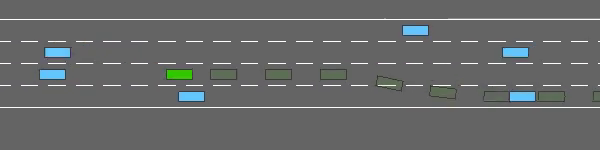
\includegraphics[width=0.7\textwidth]{img/highway-env}}    
 \end{center}

\begin{enumerate}
    \item We need to \alert{predict} the behaviours of other drivers
    \item These behaviours are {\red uncertain} and {\red non-linear}
\end{enumerate}
\vspace*{\baselineskip}
In order to efficiently capture model uncertainty, we consider the modelling framework of \alert{Linear Parameter-Varying} systems.

\end{frame}

\begin{frame}{The setting}
\begin{block}{Linear Parameter-Varying systems}
	\begin{equation*}
	\dot{x}(t)=A(\theta(t))x(t)+Bd(t)\label{eq:LPV_syst}
	\end{equation*}
	There are two sources of uncertainty:
	\begin{itemize}
		\item Parametric uncertainty $\theta(t)$
		\item External perturbations $d(t)$
	\end{itemize}
\end{block}

\centering
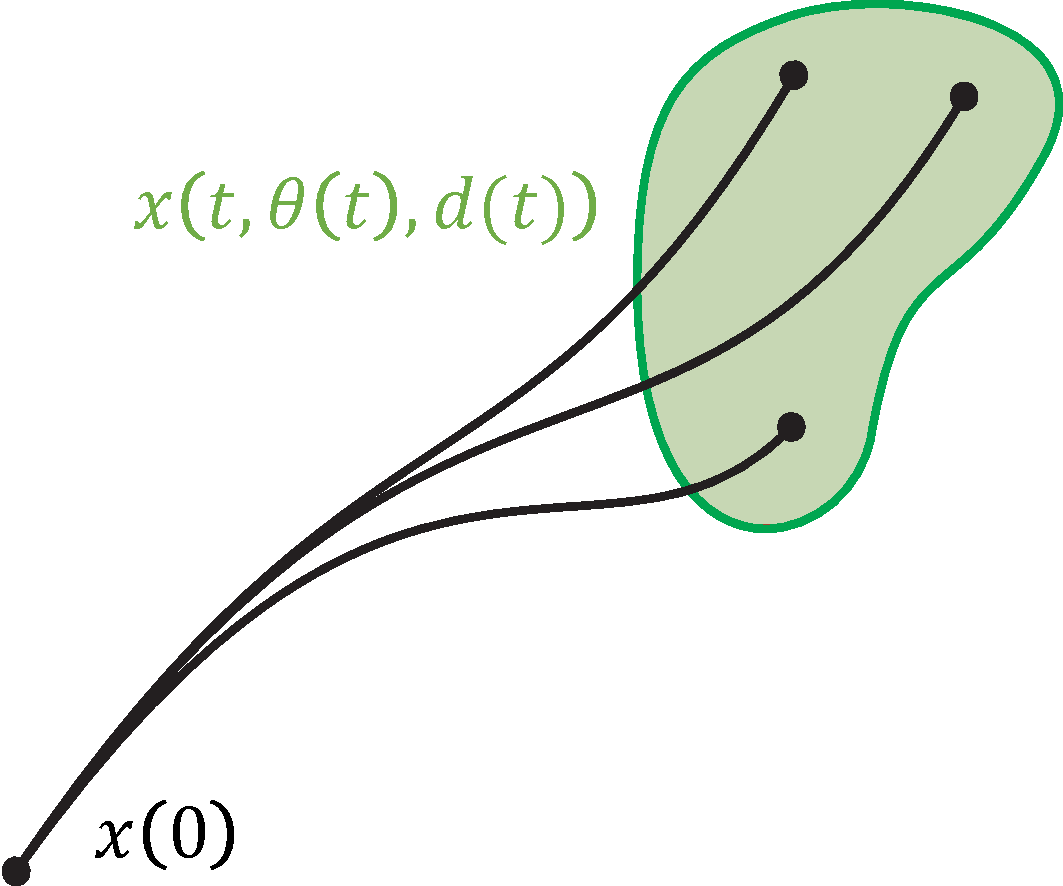
\includegraphics[width=0.45\textwidth]{img/interval-hull-0}
\end{frame}

\begin{frame}{The goal}
\begin{block}{Interval Prediction}
	Can we design an interval predictor $[\ux, \ox]$ that verifies:
	\vspace*{0.175cm}
	\begin{itemize}
		\item inclusion property: $\forall t, \ux \leq x(t) \leq \ox$;
		\item stable dynamics?
	\end{itemize}
	\vspace*{0.175cm}
	We want the predictor to be as tight as possible.

\end{block}

\centering
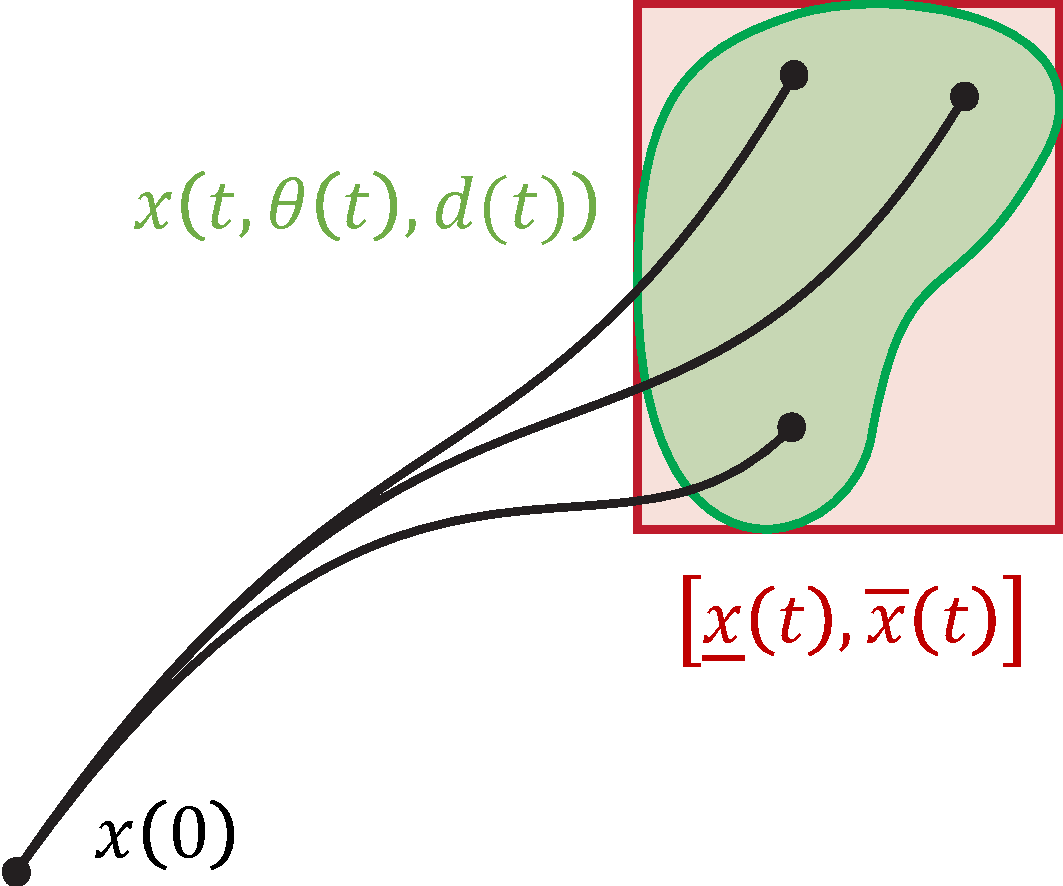
\includegraphics[width=0.45\textwidth]{img/interval-hull}
\end{frame}

\begin{frame}{Assumptions}
\begin{assumption}[Bounded trajectories]
	\begin{itemize}
		\item $\|x\|_{\infty} < \infty$
		\item $x(0)\in[\underline{x}_{0},\overline{x}_{0}]$ for some \alert{known} $\underline{x}_{0},\overline{x}_{0}\in\Real^{n}$
	\end{itemize}
\end{assumption}
\pause
\begin{assumption}[Bounded parameters]
	\begin{itemize}
		\item $\theta(t)\in\Theta$ for some \alert{known} $\Theta$
		\item The matrix function $A(\theta)$ is \alert{known}
	\end{itemize}
	\end{assumption}
\pause
\begin{assumption}[Bounded perturbations]
	\begin{itemize}
		\item $d(t)\in[\underline{d}(t),\overline{d}(t)]$ for some \alert{known} signals $\underline{d},\overline{d}\in\cL_{\infty}^{n}$
	\end{itemize}
\end{assumption}

\begin{flushright}
	How to proceed?
\end{flushright}
\end{frame}

\begin{frame}{A first idea}

Assume that $\underline{x}(t)\le x(t)\le\overline{x}(t)$, for some $t\geq0$. 
\pause
\begin{itemize}[<+->]
	\item[$\drsh$] To propagate the interval to $x(t+dt)$, we need to \\ \alert{bound $A(\theta(t))x(t)$}.
	\item[$\drsh$] Why not use \alert{interval arithmetics}?
\end{itemize}

\only<1-4>{\visible<4>{
\begin{lemma}[Image of an interval (\cite{EFRZS12})]
If $A$ a \alert{known} matrix, then
\begin{equation*}
A^{+}\underline{x}-A^{-}\overline{x}\le Ax\le A^{+}\overline{x}-A^{-}\underline{x}.\label{eq:Interval1}
\end{equation*}
where $A^+ = \max(A, 0)$ and $A^- = A-A^+$. 
\end{lemma}
}}
\only<5-6>{
\begin{lemma}[Product of intervals (\cite{EFRZS12})]
	If $A$ is \alert{unknown} but \alert{bounded} \textup{$\underline{A}\le A\le\overline{A}$},
	\begin{gather*}
	\underline{A}^{+}\underline{x}^{+}-\overline{A}^{+}\underline{x}^{-}-\underline{A}^{-}\overline{x}^{+}+\overline{A}^{-}\overline{x}^{-}\leq Ax\\
	\leq\overline{A}^{+}\overline{x}^{+}-\underline{A}^{+}\overline{x}^{-}-\overline{A}^{-}\underline{x}^{+}+\underline{A}^{-}\underline{x}^{-}. 
	\end{gather*}
\end{lemma}
}
\visible<6>{
	\begin{itemize}
		\item[\green \checkmark] Since $A(\theta)$ and the set $\Theta$ are known, \\
		we can easily compute such bounds $\underline{A} \leq A(\theta(t))\leq \overline{A}$
	\end{itemize}
}
\end{frame}


\begin{frame}{A candidate predictor}
Following this result, define the predictor:
\begin{eqnarray}
\dot{\underline{x}}(t) & = & \underline{A}^{+}\underline{x}^{+}(t)-\overline{A}^{+}\underline{x}^{-}(t)-\underline{A}^{-}\overline{x}^{+}(t)\nonumber \\
&  & +\overline{A}^{-}\overline{x}^{-}(t)+B^{+}\underline{d}(t)-B^{-}\overline{d}(t),\label{eq:IP_direct}\\
\dot{\overline{x}}(t) & = & \overline{A}^{+}\overline{x}^{+}(t)-\underline{A}^{+}\overline{x}^{-}(t)-\overline{A}^{-}\underline{x}^{+}(t)\nonumber \\
&  & +\underline{A}^{-}\underline{x}^{-}(t)+B^{+}\overline{d}(t)-B^{-}\underline{d}(t),\nonumber \\
&  & \underline{x}(0)=\underline{x}_{0},\;\overline{x}(0)=\overline{x}_{0},\nonumber
\end{eqnarray}
\pause
\begin{proposition}[Inclusion property]
	\begin{itemize}
		\item[\checkmark] The predictor \eqref{eq:IP_direct} satisfies $\ux\leq x(t)\leq \ox(t)$
	\end{itemize} 
\end{proposition}
\pause
\begin{itemize}
	\item[?] But is it stable?
\end{itemize}
\end{frame}
\begin{frame}{Motivating example}
Consider the scalar system, for all $t\geq0$:
\[
	\dot{x}(t)=-\theta(t)x(t)+d(t), \text{ where} 
	\begin{cases}
	x(0)\in[\underline{x}_{0},\overline{x}_{0}]=[1.0, 1.1],\\
	\theta(t)\in\Theta=[\underline{\theta},\overline{\theta}]=[1,2],\\
	d(t)\in[\underline{d},\overline{d}]=[-0.1,0.1],
	\end{cases}
\]
\begin{center}
\includegraphics<1>[trim={0 1.4cm 0 0.4cm}, clip, width=0.7\linewidth]{img/system}
\includegraphics<2>[trim={0 1.4cm 0 0.4cm}, clip, width=0.7\linewidth]{img/observer}
\end{center}

\begin{columns}
	\begin{column}{0.48\linewidth}
		\begin{itemize}
			\item[{\green \checkmark}] The system is always {\green stable}
		\end{itemize}
	\end{column}
	\begin{column}{0.52\linewidth}
		\begin{itemize}
			\item<2>[{\red \xmark}] The predictor \eqref{eq:IP_direct} is {\red unstable}
		\end{itemize}
	\end{column}
\end{columns}

\end{frame}

\section{Our proposed predictor}
\frame{\sectionpage}


\begin{frame}{Additional assumption}
\begin{assumption}[Polytopic Structure]
	\label{ass:a3} There exist $A_{0}$ \alert{Metzler} and $\Delta A_{0}, \cdots, \Delta A_{N}$ such that:
	\begin{gather*}
	A(\theta)=\underbrace{A_{0}}_{\substack{\text{Nominal}\\\text{dynamics}}} + \sum_{i=1}^{N}\lambda_{i}(\theta)\Delta A_{i},\quad \sum_{i=1}^{N}\underbrace{\lambda_{i}(\theta)}_{\geq 0}=1;\quad \forall\theta\in\Theta
	\end{gather*}
\end{assumption}
\centering
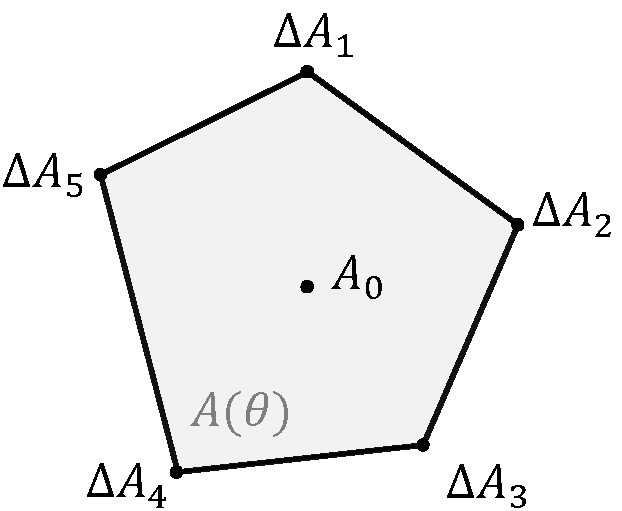
\includegraphics[width=0.42\linewidth]{img/polytope}
\end{frame}

\begin{frame}{Our proposed predictor}
Denote
\[
\Delta A_{+}=\sum_{i=1}^{N}\Delta A_{i}^{+},\;\Delta A_{-}=\sum_{i=1}^{N}\Delta A_{i}^{-},
\]
We define the predictor
\begin{eqnarray}
\alert{\dot{\underline{x}}(t)} & = & A_{0}\alert{\underline{x}(t)}-\Delta A_{+}\underline{x}^{-}(t)-\Delta A_{-}\overline{x}^{+}(t)\nonumber \\
&  & +B^{+}\underline{d}(t)-B^{-}\overline{d}(t),\nonumber\\
\alert{\dot{\overline{x}}(t)} & = & A_{0}\alert{\overline{x}(t)}+\Delta A_{+}\overline{x}^{+}(t)+\Delta A_{-}\underline{x}^{-}(t)\label{eq:IP_main} \\
&  & +B^{+}\overline{d}(t)-B^{-}\underline{d}(t),\nonumber \\
&  & \underline{x}(0)=\underline{x}_{0},\;\overline{x}(0)=\overline{x}_{0}\nonumber 
\end{eqnarray}


\begin{theorem}[Inclusion property]
	\label{thm:main}
	The predictor \eqref{eq:IP_main} ensures $\ux\leq x(t)\leq \ox$. 
\end{theorem}

\end{frame}

\begin{frame}{Stability}

\begin{theorem}[Stability]
	If there exist diagonal matrices $P$, $Q$, $Q_{+}$, $Q_{-}$, $Z_{+}$, $Z_{-}$, $\Psi_{+}$, $\Psi_{-}$, $\Psi$, $\Gamma\in\Real^{2n\times2n}$ such that the following LMIs are satisfied:
	\begin{gather*}
	P+\min\{Z_{+},Z_{-}\}>0,\;\hleb{\Upsilon\preceq0},\;\Gamma>0,\\
	Q+\min\{Q_{+},Q_{-}\}+2\min\{\Psi_{+},\Psi_{-}\}>0,
	\end{gather*}
	where \hlb{$\Upsilon = \Upsilon(A_0, \Delta A_-, \Delta A_+, \Psi_-, \Psi_+, \Psi)$}, 
	
	then the predictor \eqref{eq:IP_main} is input-to-state stable with respect to the inputs $\underline{d}$, $\overline{d}$.
\end{theorem}

\end{frame}

% \begin{frame}
% where{\footnotesize{}
% 	\begin{gather*}
% 	\Upsilon=\left[\begin{array}{cccc}
% 	\Upsilon_{11} & \Upsilon_{12} & \Upsilon_{13} & P\\
% 	\Upsilon_{12}^{\top} & \Upsilon_{22} & \Upsilon_{23} & Z_{+}\\
% 	\Upsilon_{13}^{\top} & \Upsilon_{23}^{\top} & \Upsilon_{33} & Z_{-}\\
% 	P & Z_{+} & Z_{-} & -\Gamma
% 	\end{array}\right],\\
% 	\Upsilon_{11}=\mathcal{A}^{\top}P+P\mathcal{A}+Q,\;\Upsilon_{12}=\mathcal{A}^{\top}Z_{+}+PR_{+}+\Psi_{+},\\
% 	\Upsilon_{13}=\mathcal{A}^{\top}Z_{-}+PR_{-}+\Psi_{-},\;\Upsilon_{22}=Z_{+}R_{+}+R_{+}^{\top}Z_{+}+Q_{+},\\
% 	\Upsilon_{23}=Z_{+}R_{-}+R_{+}^{\top}Z_{-}+\Psi,\;\Upsilon_{33}=Z_{-}R_{-}+R_{-}^{\top}Z_{-}+Q_{-},\\
% 	\mathcal{A}=\left[\begin{array}{cc}
% 	A_{0} & 0\\
% 	0 & A_{0}
% 	\end{array}\right],\;R_{+}=\left[\begin{array}{cc}
% 	0 & -\Delta A_{-}\\
% 	0 & \Delta A_{+}
% 	\end{array}\right],\;R_{-}=\left[\begin{array}{cc}
% 	\Delta A_{+} & 0\\
% 	-\Delta A_{-} & 0
% 	\end{array}\right],
% 	\end{gather*}
% }
% \end{frame}

\begin{frame}{Sketch of proof}
\begin{enumerate}
	\item Define the extended state vector as $X=[\underline{x}^{\top}\;\;\overline{x}^{\top}]^{\top}$
	\item It follows the dynamics $$\dot{X}(t)=\mathcal{A}X(t)+R_{+}X^{+}(t)-R_{-}X^{-}(t)+\delta(t)$$
	$$\mathcal{A}=\left[\begin{array}{cc}
    A_{0} & 0\\
    0 & A_{0}
    \end{array}\right]
    	\;R_{+}=\left[\begin{array}{cc}
    0 & -\Delta A_{-}\\
    0 & \Delta A_{+}
    \end{array}\right],\;R_{-}=\left[\begin{array}{cc}
    \Delta A_{+} & 0\\
    -\Delta A_{-} & 0
    \end{array}\right]$$
	\item Consider a candidate Lyapunov function:
	\begin{gather*}
	V(X)=X^{\top}PX+X{}^{\top}Z_{+}X^{+}-X^{\top}Z_{-}X^{-}
	\end{gather*}
	\item $V(X)$ is positive definite provided that
	$
	P+\min\{Z_{+},Z_{-}\}>0,
	$
	\item Check on which condition we have $\dot{V}(X) \leq 0$
\end{enumerate}
\end{frame}

\begin{frame}{Back to our motivating example}
Recall the scalar system:
\[
\dot{x}(t)=-\theta(t)x(t)+d(t), \text{ where} 
\begin{cases}
x(0)\in[\underline{x}_{0},\overline{x}_{0}]=[1.0, 1.1],\\
\theta(t)\in\Theta=[\underline{\theta},\overline{\theta}]=[1,2],\\
d(t)\in[\underline{d},\overline{d}]=[-0.1,0.1],
\end{cases}
\]
\begin{center}
	\includegraphics<1>[trim={0 1.4cm 0 0.4cm}, clip, width=0.7\linewidth]{../img/predictor}
\end{center}

\begin{columns}
	\begin{column}{0.48\linewidth}
		\begin{itemize}
			\item[{\green \checkmark}] The system is always {\green stable}
		\end{itemize}
	\end{column}
	\begin{column}{0.52\linewidth}
		\begin{itemize}
			\item[{\green \checkmark}] The predictor \eqref{eq:IP_main} is {\green stable}
		\end{itemize}
	\end{column}
\end{columns}

\end{frame}


\section{Application to autonomous driving}

 \frame{\sectionpage}
 
 \begin{frame}{A multi-agent system}
 
 \begin{center}
 \href{https://github.com/eleurent/highway-env\#highway}{
 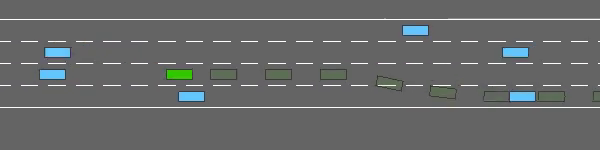
\includegraphics[width=0.7\textwidth]{img/highway-env}}    
 \end{center}
 
 $$\dot{z}_i=f_i(Z,\theta_i),\;i=\overline{1,N},$$ where
 
 \begin{itemize}
 	\item $z_i = [x_i, y_i, v_i, \psi_i]^\top\in\Real^4$ is the state of an agent
 	\item $\theta_i\in\Real^5$ is the corresponding unknown behavioural parameters
 	\item $Z = [z_1,\dots,z_N]^\top\in\Real^{4N}$  is the joint state of the traffic
 	\item $\theta=[\theta_1,\dots,\theta_N]^\top \in \Pi\subset\Real^{5N}$	
 \end{itemize}
\end{frame}

\begin{frame}{Kinematics}
\begin{center}
\begin{tabular}{ccl}
    \toprule
    \multirow{3}{*}{States} & $(x_i, y_i)$ & position \\
    & $v_i$ & longitudinal velocity \\
    & $\psi_i$ & yaw angle \\
    \midrule
    \multirow{2}{*}{Controls} & $a_i$ & longitudinal acceleration \\
    & $\beta_i$ & slip angle at the center of gravity \\
    \bottomrule
\end{tabular}
\end{center}
Each vehicle follows the Kinematic Bicycle Model:
\begin{align}
	\dot{x}_i &= v_i\cos(\psi_i), \nonumber\\
	\dot{y}_i &= v_i\sin(\psi_i), \nonumber\\
	\dot{v}_i &= a_i, \nonumber\\
	\dot{\psi}_i &= \frac{v_i}{l}tan(\beta_i), \nonumber
\end{align}
\end{frame}

\begin{frame}{Longitudinal control}
A linear controller using three features inspired from the intelligent driver model (IDM) [\cite{Treiber2000}].

	\begin{equation*}
	a_i = \begin{bmatrix}
	\theta_{i,1} & \theta_{i,2} & \theta_{i,3}
	\end{bmatrix} \begin{bmatrix}
	v_0 - v_i \\
	-(v_{f_i}-v_i)^- \\
	-(x_{f_i} - x_i - (d_0 + v_iT))^- \\
	\end{bmatrix},
	\label{eq:theta_a}
	\end{equation*}
	%where $v_0, d_0$ and $T$ respectively denote the speed limit, jam distance and time gap given by traffic rules, and $f_i$ is the index of the leading vehicle of vehicle $i$.
	where
	\begin{center}
	\begin{tabular}{cl}
    \toprule
    $v_0$ & speed limit \\
    $d_0$ & jam distance \\
    $T$ & time gap \\
    $f_i$ & index of vehicle $i$'s front vehicle\\
    \bottomrule
    \end{tabular}    
	\end{center}
	
\end{frame}

\begin{frame}{Lateral Control}
A cascade controller of lateral position $y_i$ and heading $\psi_i$:
\begin{align}
\label{eq:heading-command}
\dot{\psi}_i &= \theta_{i,5}\left(\psi_{L_i}+\sin^{-1}\left(\frac{\tilde{v}_{i,y}}{v_i}\right)-\psi_i\right),\\
\tilde{v}_{i,y} &= \theta_{i,4} (y_{L_i}-y_i). \nonumber
\end{align}
We assume that the drivers choose their steering command $\beta_i$ such that \eqref{eq:heading-command} is always achieved: $\beta_i = \tan^{-1}(\frac{l}{v_i}\dot{\psi}_i)$.
\end{frame}

\begin{frame}{LPV Formulation}

We linearize trigonometric operators around $y_i=y_{L_i}$ and $\psi_i=\psi_{L_i}$.

This yields the following longitudinal dynamics:
\begin{align*}
\dot{x}_i &= v_i,\\
\dot v_i &= \theta_{i,1} (v_0 - v_i) + \theta_{i,2} (v_{f_i} - v_i) + \theta_{i,3}(x_{f_i} - x_i - d_0 - v_i T),
\end{align*}
where $\theta_{i,2}$ and $\theta_{i,3}$ are set to $0$ whenever the corresponding features are not active.
\end{frame}

\begin{frame}{LPV Formulation}
$$\dot{Z} = A(\theta)(Z-Z_c) + d.$$ For example, in the case of two vehicles only:
\begin{equation*}
Z = \begin{bmatrix}
x_i \\
x_{f_i} \\
v_i \\
v_{f_i} \\
\end{bmatrix}
,\quad
Z_c = \begin{bmatrix}
-d_0-v_0 T \\
0 \\
v_0\\
v_0 \\
\end{bmatrix}
,\quad
d = \begin{bmatrix}
v_0 \\
v_0 \\
0\\
0\\
\end{bmatrix}
\end{equation*}

\begin{equation*}
A(\theta)
=
\begin{blockarray}{ccccc}
& i & f_i & i & f_i \\
\begin{block}{c[cccc]}
i & 0 & 0 & 1 & 0 \\
f_i & 0 & 0 & 0 & 1 \\
i & -\theta_{i,3} & \theta_{i,3} & -\theta_{i,1}-\theta_{i,2}-\theta_{i,3} & \theta_{i,2} \\
f_i & 0 & 0 & 0 & -\theta_{f_i,1} \\
\end{block}
\end{blockarray}
\end{equation*}
\end{frame}

\begin{frame}{LPV Formulation}
The lateral dynamics are in a similar form:
\begin{equation*}
\begin{bmatrix}
\dot{y}_i \\
\dot{\psi}_i \\
\end{bmatrix}
=
\begin{bmatrix}
0 & {\red v_i} \\
-\frac{\theta_{i,4} \theta_{i,5}}{\red v_i} & -\theta_{i,5}
\end{bmatrix}
\begin{bmatrix}
y_i - y_{L_i} \\
\psi_i - \psi_{L_i}
\end{bmatrix}
+
\begin{bmatrix}
v_i\psi_{L_i} \\
0
\end{bmatrix}
\end{equation*}
Here, the dependency in {\red $v_i$} is seen as an uncertain parametric dependency, \emph{i.e.} \alert{$\theta_{i,6}=v_i$}, with constant bounds assumed for $v_i$ using an overset of the longitudinal interval predictor.
\end{frame}

\begin{frame}{Results}
\centering
\vspace*{\baselineskip}
\href{https://eleurent.github.io/interval-prediction/\#direct-interval-predictor}{
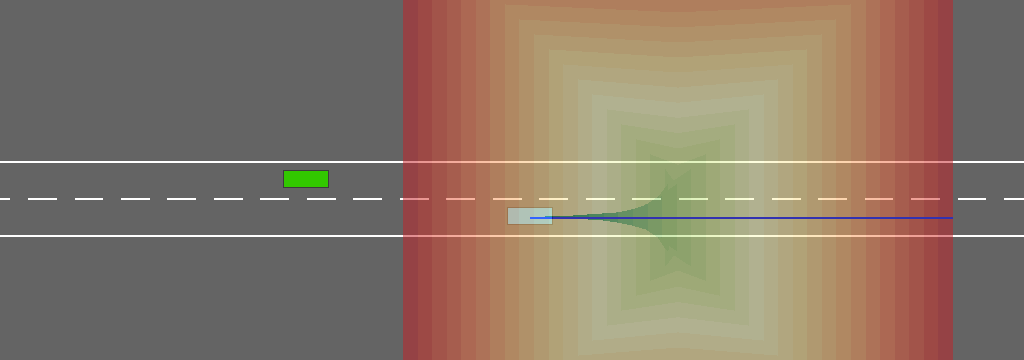
\includegraphics[width=0.75\textwidth]{../img/driving_observer.png}}

The naive predictor \eqref{eq:IP_direct} quickly diverges

\href{https://eleurent.github.io/interval-prediction/\#novel-interval-predictor}{
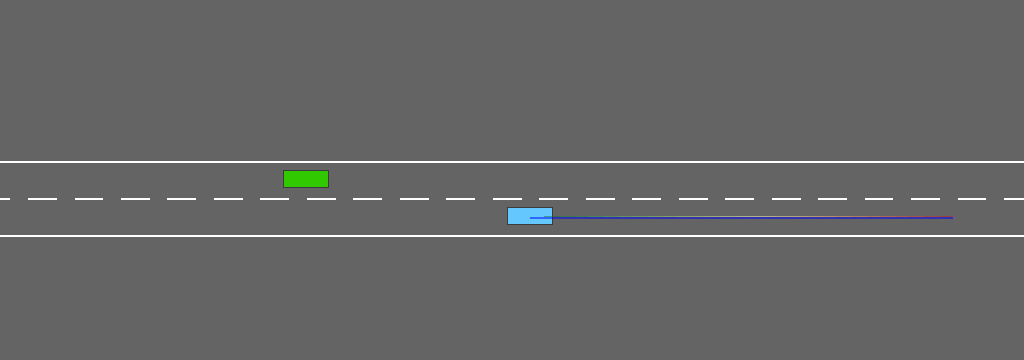
\includegraphics[width=0.75\textwidth]{../img/driving_predictor.png}}

The proposed predictor \eqref{eq:IP_main} remains stable
\end{frame}

\begin{frame}{Results}
\centering
\vspace*{\baselineskip}
\href{https://eleurent.github.io/interval-prediction/\#novel-interval-predictor}{
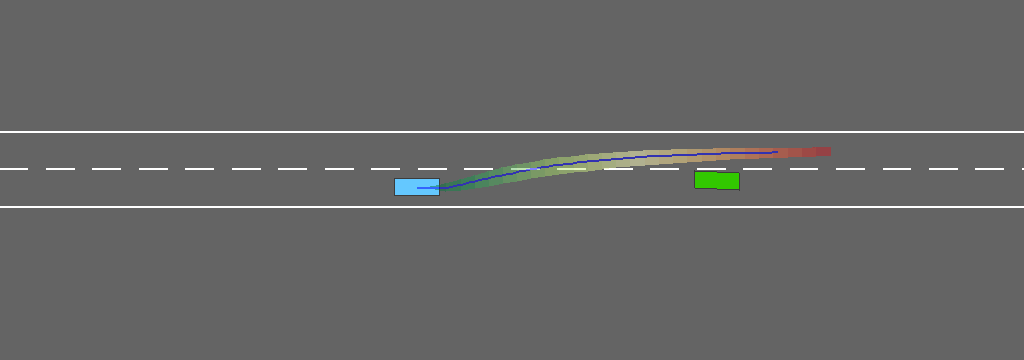
\includegraphics[width=0.75\textwidth]{../img/lane_change_predictor.png}}

Prediction during a lane change maneuver

\href{https://eleurent.github.io/interval-prediction/\#right-hand-traffic}{
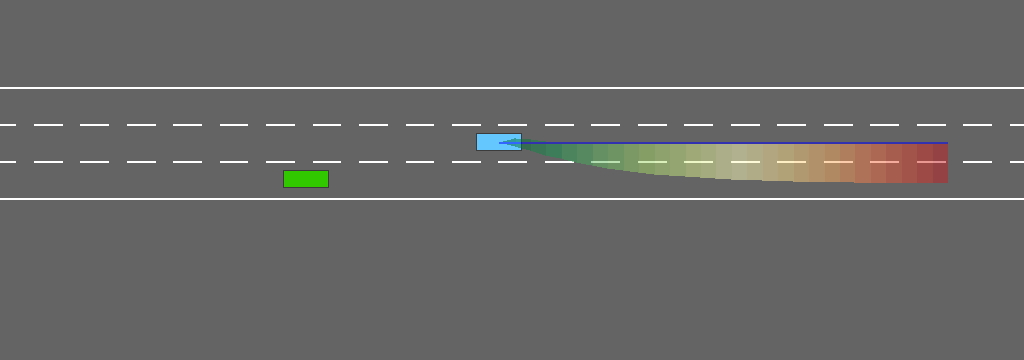
\includegraphics[width=0.75\textwidth]{../img/overtake.png}}

Prediction with uncertainty in the followed lane $L_i$
\end{frame}

\begin{frame}{Conclusion}
    
    \begin{block}{Problem formulation}
    \begin{itemize}
        \item Prediction of an {\red uncertain non-linear} system
        \item[\red $\drsh$] Within the \alert{LPV} framework
        \item[\red $\drsh$] Design of an \alert{interval} predictor $[\underline{x}(t), \overline{x}(t)]$?
    \end{itemize}
    \end{block}
    
    \begin{block}{Proposed solution}
    \begin{itemize}
        \item Direct prediction with interval arithmetics is \alert{valid} but {\red unstable}
        \item[\red $\drsh$] Assume \alert{polytopic uncertainty} structure around a nominal $A_0$
        \item[\red $\drsh$] \alert{Ensure stability} using a Luyapunov function in an LMI form
    \end{itemize}
    \end{block}
    
    \begin{block}{Application}
    \begin{itemize}
        \item Joint prediction of coupled traffic dynamics
        \item Can be used as a building block for robust planning
    \end{itemize}
    \end{block}
\end{frame}
\end{document}
